\documentclass{article}
\usepackage{amsmath, tcolorbox, sfmath, enumerate, pgfplots, multicol}
\renewcommand{\familydefault}{\sfdefault}
\pgfplotsset{compat=newest}
\tikzset{>=stealth}
\tikzstyle{input} = [circle, text centered, radius = 1cm, draw = black]
\tikzstyle{function} = [rectangle, text centered, minimum width = 2cm, minimum height = 1cm, draw = black]
\usepackage[top = 0.25in, bottom = 0.25in, left = 1.25in, right = 1.5in]{geometry}
\pagestyle{empty}
\raggedright

\newcounter{example}[section]
\newenvironment{example}[1][]{\refstepcounter{example}\par\medskip
   {\color{red}\textbf{Example~\theexample. #1}}}{\medskip}

\begin{document}

\section*{Operations and Compositions of Functions}

\begin{tcolorbox}[colframe=orange!70!white, coltitle=black, title=\textbf{Summary}]
\begin{enumerate}
    \item We can add, subtract, multiply, and divide outputs of functions just like we can with real numbers.
    \item Revenue = Products sold $\times$ unit price per product.
    \item Profit = Revenue $-$ Cost.
    \item The break-even point is when revenue = cost.
    \item Function compositions involve plugging one function into another.
\end{enumerate}
\end{tcolorbox}
\vspace{0.5in}

\subsection*{Operations on Functions}

For functions $f(x)$ and $g(x)$:
\begin{itemize}
    \item $(f + g)(x) = f(x) + g(x)$
    \item $(f - g)(x) = f(x) - g(x)$
    \item $(f \cdot g)(x) = f(x) \cdot g(x)$
    \item $\left(\frac{f}{g}\right)(x) = \frac{f(x)}{g(x)}, \text{ provided that $g(x) \neq 0$}$
\end{itemize}
\vspace{1in}

\begin{example}
Let $f(x) = x^2 + x - 3$ and $g(x) = 4x + 2$. Evaluate the following.
\begin{multicols}{4}
\begin{enumerate}[(a)]
    \item $(f + g)(1)$
    \item $(f - g)(1)$
    \item $(f \cdot g)(1)$
    \item $\left(\frac{f}{g}\right)(1)$
\end{enumerate}
\end{multicols}
\end{example}
\vspace{1.5in}

\subsection*{Functions of Business}


The {\color{blue}\textbf{price-demand function}} $p$ gives the price $p(x)$ at which people buy exactly $x$ units of a product. 

The cost $C(x)$ of producing $x$ units of a product is given by the cost function
\[
C(x) = (\text{variable costs}) \cdot (\text{units produced}) + (\text{fixed costs})
\]
\vfill 
The revenue $R(x)$ of producing $x$ units is
\begin{align*}
R(x) &= (\text{quantity sold}) \cdot (\text{unit price}) \\
&= x \cdot p(x)
\end{align*}

\vfill 
\newpage 

\begin{example}
An online streaming service knows from past sales records that the weekly number of units demanded $x$ of their content is shown below:
\begin{center}
    \begin{tabular}{cc}
        \textbf{Demand} $\pmb{x}$ & \textbf{Price} $\pmb{p(x)}$ \\ \hline 
        10 & \textdollar 25 \\
        30 & \textdollar 20 \\
    \end{tabular}
\end{center}
\begin{enumerate}[(a)]
    \item Find the linear price function $p$, in slope-intercept form.  \vspace{1.25in}
    \item Determine the revenue function, $R(x)$.   \vspace{1in}
    \item Use a graphing utility to find the maximum point of the revenue function.   \vspace{2in}
\end{enumerate}
\end{example}

The profit is given by
\begin{align*}
    \text{Profit} &= \text{revenue} - \text{cost} \\
    P(x) &= R(x) - C(x) \\
\end{align*}

\newpage 

\begin{example}
A company makes designer ties. It determines the weekly cost and revenue functions, in dollars, for producing and selling $x$ designer ties are
\[
C(x) = 30x + 50 \quad \text{and} \quad R(x) = 90x - x^2
\]
\begin{enumerate}[(a)]
    \item Determine the profit function $P$.    \vspace{1.5in}
    \item Find the maximum point of the profit function.    \vspace{2in}
\end{enumerate}
\end{example}

The {\color{blue}\textbf{break-even point}} is when revenue equals cost: $R(x) = C(x)$.
\vspace{1.5in}

\begin{example}
Suppose a company's revenue and cost functions are $R(x) = 25x-0.25x^2$ and $C(x) = 2x+5$. Find and interpret the break-even point.
\end{example}

\newpage 

\subsection*{Compositions of Functions}

We can also use the output of one function as input into another.    \newline\\

The \textbf{composition of a function \textit{f} and \textit{g}}, denoted $(f \circ g)(x)$, is
\newline\\

\[  (f \circ g)(x) = f(g(x))    \] 
\newline\\

where we plug $g(x)$ into the variable for $f(x)$.  
\vfill 


The diagram below shows the result of $f(g(8))$, in which $g(x)=2x+3$ and $f(x)=x^2$.  
\begin{enumerate}
    \item Evaluate $g(8)$ to get $2(8) + 3$, or 19.  
    \item Evaluate $f(19)$ to get $19^2$, or 361. 
\end{enumerate}
\vspace{0.25in}

\begin{center}
    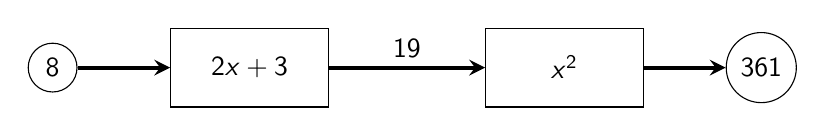
\begin{tikzpicture}[node distance = 2.5cm]
    \node (inputVal) [input] {8};
    \node (fx) [function, right of = inputVal] {$2x + 3$};
    \node (gx) [function, right of = fx, node distance = 4cm] {$x^2$};
    \node (outputVal) [input, right of = gx] {361};
    \node at (4.5,0) [anchor = south] {19};
    
    \draw [->, >=stealth, line width = 1.5] (inputVal) -- (fx);
    \draw [->, >=stealth, line width = 1.5] (fx) -- (gx);
    \draw [->, >=stealth, line width = 1.5] (gx) -- (outputVal);
    \end{tikzpicture}
\end{center}  
\vfill 

\begin{example}
Suppose $f(x) = \frac{3}{x}$ and $g(x) = 2x-1$. Evaluate each.
\begin{multicols}{2}
\begin{enumerate}[(a)]
    \item $f(g(6))$
    \item $g(f(6))$
\end{enumerate}
\end{multicols}
\end{example}
\vfill 

\newpage 

We will later use compositions with the Chain Rule. \newline\\

An important part of that will be {\color{blue}\textbf{decomposing}} a composite function into simpler functions.
\vspace{1.5in}

\begin{example}
Determine functions $f$ and $g$ for each composition such that $f(g(x)) = h(x)$.
\begin{multicols}{2}
\begin{enumerate}[(a)]
    \item $h(x) = \sqrt{(x+5)^3}$
    \item $h(x) = (5x^3 + 6)^2$
\end{enumerate}
\end{multicols}
\end{example}


\end{document}
